\section{Geometric view of systems of equations}
\label{sec:systems-geometric}

\begin{outcome}
\begin{enumerate}
\item[A.] Relate the types of solution sets of a system of two (three)
variables to the intersections of lines in a plane (the intersection of
planes in three-dimensional space)
\end{enumerate}
\end{outcome}

As you may remember, linear equations like $2x+3y=6$ can be graphed as
straight lines in the coordinate plane. We say that this equation is
in two variables, in this case $x$ and $y$.  Suppose you have two such
equations, each of which can be graphed as a straight line, and consider
the resulting graph of two lines. What would it mean if there exists a
point of intersection between the two lines? This point, which lies on
{\em both \em} graphs, gives $x$ and $y$ values for which both
equations are true. In other words, this point gives the ordered pair
($x,y$) that satisfies both equations.  If the point $\tup{x, y
}$ is a point of intersection, we say that $\tup{x, y }$
is a \textbf{solution} to the two equations. In linear algebra, we
often are concerned with finding the solution(s) to a system of
equations, if such solutions exist.  First, we consider graphical
representations of solutions and later we will consider the algebraic
methods for finding solutions.

When looking for the intersection of two lines in the plane, several situations may arise. The following picture demonstrates the possible situations
when considering two equations (two lines in the plane) involving two variables.

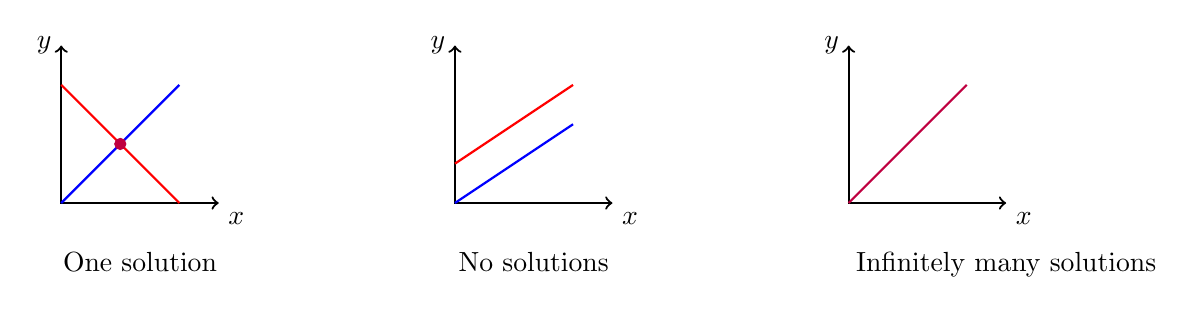
\begin{tikzpicture}
\draw[thick, <->](0,2)--(0,0)--(2,0);
\draw[thick, red](0,1.5)--(1.5,0);
\draw[thick, blue](0,0)--(1.5,1.5);
\draw[fill, purple](0.75,0.75) circle [radius=2pt];
\node[below right] at (2,0){$x$};
\node[left] at (0,2){$y$};
\node[below] at (1,-0.5){One solution};

\draw[thick, <->](5,2)--(5,0)--(7,0);
\draw[thick, red](5,0.5)--(6.5, 1.5);
\draw[thick, blue](5,0)--(6.5,1);
\node[below right] at (7,0){$x$};
\node[left] at (5,2){$y$};
\node[below] at (6,-0.5){No solutions};

\draw[thick, <->](10,2)--(10,0)--(12,0);
\draw[thick, purple](10,0)--(11.5, 1.5);
\node[below right] at (12,0){$x$};
\node[left] at (10,2){$y$};
\node[below] at (12,-0.5){Infinitely many solutions};
\end{tikzpicture}


In the first diagram, there is a unique point of
intersection, which means that there is only one (unique) solution to the two equations. 
In the second, there are no points of intersection and  no solution. There is no solution because the two lines are parallel and they never intersect.
The third situation that can occur, as demonstrated in diagram three, is that the two lines are really the same line. For
example, $x+y=1$ and $2x+2y=2$ are two equations that yield the
same line when graphed. In this case there are infinitely many points that are
solutions of these two equations, as every ordered pair which is on the graph of
the line satisfies both equations. 

When considering linear systems of equations, there are always three
possibilities for the number of solutions: there is exactly one
solution, there are infinitely many solutions, or there is no
solution.  When we speak of {\em solving} a system of equations, we
usually mean finding {\em all} of its solutions. This can mean finding
one solution (if the solution is unique), finding infinitely many
solutions, or finding that there is no solution.

\begin{example}{A graphical solution}{graphicalsoln}
Use a graph to solve the following system of equations \:
\begin{equation*}
\begin{array}{r@{~}c@{~}l}
x+y&=&3 \\
y-x&=&5.
\end{array}
\end{equation*}
\end{example} 

\begin{solution} Through graphing the above equations and identifying the point of intersection, we can find the solution(s). Remember that we must have either one solution, infinitely many, or no solutions at all. 
 The following graph shows the two equations,
as well as the intersection. Remember, the point of intersection represents the solution of
the two equations, or the $\tup{x,y}$ which satisfy both equations. In this case,
there is one point of intersection at $\tup{-1, 4 }$ which means we have one unique solution, $x = -1$, $y = 4$.

\begin{center}
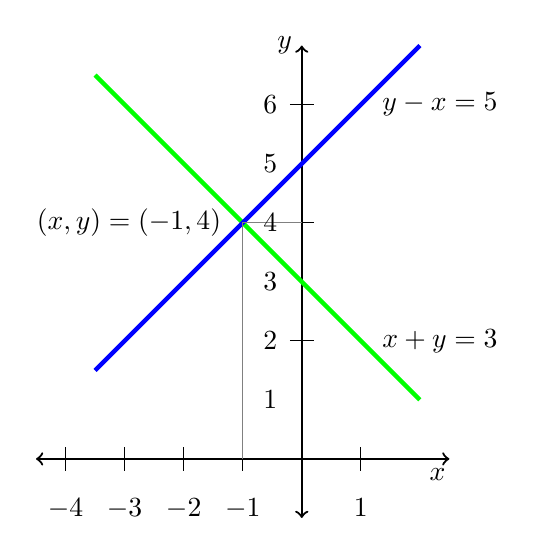
\begin{tikzpicture}[scale=0.75]
\draw[thick, <->](-4.5,0) -- (2.5,0);
\draw[thick, <->](0,-1) -- (0,7);
\draw(-4,-0.2) -- (-4,0.2);
\draw(-3,-0.2) -- (-3,0.2);
\draw(-2,-0.2) -- (-2,0.2);
\draw(-1,-0.2) -- (-1,0.2);
\draw(1,-0.2) -- (1,0.2);
\draw(-0.2,2) -- (0.2,2);
\draw(-0.2,4) -- (0.2,4);
\draw(-0.2,6) -- (0.2,6);
\draw[green, ultra thick, domain=-3.5:2] plot (\x, {3-\x});
\draw[blue, ultra thick, domain=-3.5:2] plot (\x, {\x+5});
\node[right] at (1.2,2){$x+y=3$};
\node[right] at (1.2,6){$y-x=5$};
\draw[help lines](-1,0)--(-1,4)--(0,4);
\node[below] at (-4,-0.5){$-4$};
\node[below] at (-3,-0.5){$-3$};
\node[below] at (-2,-0.5){$-2$};
\node[below] at (-1,-0.5){$-1$};
\node[below] at (1,-0.5){$1$};
\node[left] at (-0.25,1){$1$};
\node[left] at (-0.25,2){$2$};
\node[left] at (-0.25,3){$3$};
\node[left] at (-0.25,4){$4$};
\node[left] at (-0.25,5){$5$};
\node[left] at (-0.25,6){$6$};
\node[below right] at (2,0){$x$};
\node[left] at (0,7){$y$};
\node[left=1ex] at (-1,4){$(x,y) = (-1,4)$};
\end{tikzpicture}
\vspace{-2ex}
\end{center}
\end{solution}

In the above example, we investigated the intersection point of two equations in two variables, $x$ and $y$. Now we will consider 
the graphical solutions of three equations in two variables.

Consider a system of three equations in two variables. Again, these equations can be graphed as
straight lines in the plane, so that the resulting graph contains three straight lines. Recall the three possibilities for the number of solutions: no solution, one solution, and infinitely many solutions.
With three lines, there are more complex ways of achieving these situations. For example, you can imagine the case of three intersecting
lines having no common point of intersection. Perhaps you can also imagine three intersecting lines
which do intersect at a single point. These two situations are illustrated below. 

\begin{center}
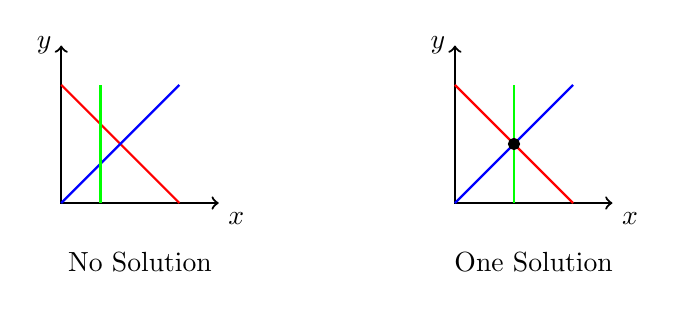
\begin{tikzpicture}
\draw[thick, <->](0,2)--(0,0)--(2,0);
\draw[thick, red](0,1.5)--(1.5,0);
\draw[thick, blue](0,0)--(1.5,1.5);
\draw[thick, green](0.5,0)--(0.5,1.5);
\node[below right] at (2,0){$x$};
\node[left] at (0,2){$y$};
\node[below] at (1,-0.5){No Solution};

\draw[thick, <->](5,2)--(5,0)--(7,0);
\draw[thick, red](5,1.5)--(6.5,0);
\draw[thick, blue](5,0)--(6.5,1.5);
\draw[thick, green](5.75,0)--(5.75,1.5);
\draw[fill](5.75,0.75) circle [radius=2pt];
\node[below right] at (7,0){$x$};
\node[left] at (5,2){$y$};
\node[below] at (6,-0.5){One Solution};
\end{tikzpicture}
\end{center}

Consider the first picture above. While all three lines intersect with one another, there is no common point of intersection
where all three lines meet at one point. Hence, there is no solution to the three equations. Remember, a solution is a point $\tup{x, y }$
which satisfies \textbf{all} three equations.
In the case of the second picture, the lines intersect at a common point. This means that there is one solution to the three equations whose graphs are the
given lines. 
You should take a moment now to draw the graph of a system which results in three parallel lines. Next, try the graph of three identical lines.  Which type of solution is represented in each of these graphs?

We have now considered the graphical solutions of systems of two equations in two variables, as well as three equations in two variables. However, there is no reason to limit our investigation to equations in two variables. We will now consider equations in three variables.

You may recall that equations in three variables, such as $2x+4y-5z=8$, form a plane. Above, we were looking for intersections of lines in order to 
identify any possible solutions. When graphically solving systems of equations in three variables, we look for 
intersections of planes. These points of intersection give the $\tup{x, y, z }$ that satisfy all the equations 
in the system.  What types of solutions are possible when working with three variables?
 Consider the following picture involving two planes, which are given by two 
equations in three variables.

\begin{picture}(1,120)
\put(80,30){\begin{picture}(1,1) %\thicklines
\setlength{\unitlength}{.3pt} \put(0,0){\line(1,0){300}}
\put(0,0){\line(1,1){75}}\put(300,150){\line(1,0){150}}\put(450,150){\line(-1,-1){150}
}\put(150,0){\line(1,1){150}}\put(150,0){\line(-1,1){100}}\put(50,100){\line(1,1){150}}
\put(200,250){\line(1,-1){100}}\put(75,75){\qbezier[14](0,0)(37.5,37.5)(75,75)}
\put(150,150){\qbezier[14](0,0)(75,0)(150,0)}\put(300,150){\qbezier[14](0,0)(37.5,-37.5)(75,-75)}
\put(375,75){\line(1,-1){20}}\put(395,55){\line(-1,-1){150}}
\put(150,0){\line(1,-1){95}}
\end{picture}}
\end{picture}

Notice how these two planes intersect in a line. This means that the points $\tup{x,y,z}$ on this line
satisfy both equations in the system. Since the line contains infinitely many points, this system has infinitely many solutions.

It could also happen that the two planes fail to intersect. However, is it possible to have two planes intersect at a single point? Take a moment to attempt drawing this situation, and convince yourself that it is 
not possible! This means that when we have only two equations in three variables, there is no way to have a unique solution! Hence, the only possibilities for the number of solutions of two equations in three variables are no solution or infinitely many solutions. 

Now imagine adding a third plane. In other words, consider three equations in three variables. What types of solutions are now possible? Consider the following diagram. 

\begin{picture}(1,120)
\put(80,30){\begin{picture}(1,1) %\thicklines
\setlength{\unitlength}{.3pt} \put(0,0){\line(1,0){300}}
\put(0,0){\line(1,1){50}}\put(300,150){\line(1,0){150}}\put(450,150){\line(-1,-1){150}
}\put(150,0){\line(1,1){150}}\put(150,0){\line(-1,1){100}}\put(50,100){\line(1,1){150}}
\put(200,250){\line(1,-1){50}}
\put(250,200){\qbezier[3](0,0)(12.5,-12.5)(25,-25)}
\put(275,175){\line(1,-1){25}}
\put(50,50){\qbezier[18](0,0)(50,50)(100,100)}
\put(150,150){\qbezier[14](0,0)(75,0)(150,0)}\put(300,150){\qbezier[14](0,0)(37.5,-37.5)(75,-75)}
\put(375,75){\line(1,-1){20}}\put(395,55){\line(-1,-1){150}}
\put(150,0){\line(1,-1){95}}\put(100,50){\line(1,1){150}}\put(100,50){\line(-1,0){120}}
\put(-20,50){\line(1,1){150}}\put(130,200){\line(1,0){20}}
\put(140,200){\qbezier[10](0,0)(50,0)(110,0)}\put(250,200){\line(1,0){50}}
\put(300,200){\line(-1,-1){150}} \put(150,50){\line(-1,0){50}}
\put(320,230){\vector(-1,-1){30}}\put(325,230){New Plane}
\end{picture}}
\end{picture}

In this diagram, there is no point which lies in all three planes. There is no intersection between \textbf{all} three planes
so there is no solution. The picture
illustrates the situation in which the line of intersection of the new plane
with one of the original planes forms a line parallel to the line of
intersection of the first two planes. However, in three dimensions, it is
possible for two lines to fail to intersect even though they are not
parallel. Such lines are called \textbf{skew lines}\index{skew lines}.

Recall that when working with two equations in three variables, it was not possible to have a unique solution. Is it possible 
when considering three equations in three variables? In fact, it is possible, and we demonstrate this situation in the following picture.

\begin{picture}(1,120)
\put(90,30){\begin{picture}(1,1) %\thicklines
\setlength{\unitlength}{.3pt} \put(0,0){\line(1,0){300}}
\put(0,0){\line(1,1){75}}
%\put(300,150){\line(1,0){150}}
\put(300,150){\qbezier[4](0,0)(25,0)(50,0)}
\put(350,150){\line(1,0){100}}
 \put(450,150){\line(-1,-1){150}}
\put(150,0){\line(1,1){50}}
\put(200,50){\qbezier[14](0,0)(50,50)(100,100)}
\put(150,0){\line(-1,1){100}}\put(50,100){\line(1,1){150}}
%\put(200,250){\line(1,-1){100}}
\put(200,250){\qbezier[14](0,0)(50,-50)(100,-100)}
\put(75,75){\qbezier[14](0,0)(37.5,37.5)(75,75)}
\put(150,150){\qbezier[14](0,0)(75,0)(150,0)}\put(300,150){\qbezier[14](0,0)(37.5,-37.5)(75,-75)}
\put(375,75){\line(1,-1){20}}
 \put(395,55){\line(-1,-1){45}}
 \put(350,10){\qbezier[6](0,0)(-27,-27)(-60,-60)}
 \put(290,-50){\line(-1,-1){45}}
\put(150,0){\line(1,-1){95}}\put(200,50){\line(0,1){200}}\put(200,50){\line(1,0){150}}
\put(200,50){\qbezier[10](0,0)(-50,0)(-100,0)}\put(100,50){\line(-1,0){50}}
\put(50,50){\line(0,1){200}} \put(350,50){\line(0,1){200}}
\put(350,250){\line(-1,0){300}} \put(200,50){\circle*{5}}
\put(350,50){\line(0,-1){100}}\put(200,50){\qbezier[4](0,0)(0,-25)(0,-50)}
\put(200,0){\line(0,-1){50}} \put(200,-50){\line(1,0){150}}
\put(200,-50){\line(-1,0){150}} \put(50,-50){\line(0,1){50}}
\put(50,0){\qbezier[4](0,0)(0,25)(0,50)}
\put(400,250){\vector(-1,-1){50}} \put(405,250){New Plane}
\end{picture}}
\end{picture}

In this case, the three planes have a single point of intersection. 
Can you think of other possibilities? Another is that the
three planes could intersect in a line, resulting in infinitely many solutions, as in the following diagram.

\begin{picture}(1,120)
\put(80,30){\begin{picture}(1,1) %\thicklines
\setlength{\unitlength}{.3pt} \put(0,0){\line(1,0){300}}
\put(0,0){\line(1,1){75}}
 %\put(300,150){\line(1,0){150}}
 \put(450,150){\line(-1,0){83.333}}
 \put(300,150){\qbezier[6](0,0)(33,0)(66,0)}
\put(450,150){\line(-1,-1){150}
}\put(150,0){\line(1,1){150}}\put(150,0){\line(-1,1){100}}\put(50,100){\line(1,1){150}}
\put(200,250){\line(1,-1){100}}\put(75,75){\qbezier[14](0,0)(37.5,37.5)(75,75)}
\put(150,150){\qbezier[14](0,0)(75,0)(150,0)}\put(300,150){\qbezier[14](0,0)(37.5,-37.5)(75,-75)}
\put(375,75){\line(1,-1){20}}\put(395,55){\line(-1,-1){150}}
\put(150,0){\line(1,-1){95}}\put(150,0){\line(-3,-1){90}}
\put(60,-30){\line(1,1){30}}
\put(150,0){\line(3,1){100}}\put(250,33.333){\line(1,1){150}}
\put(400,183.333){\line(-3,-1){100}}
\end{picture}}
\end{picture}

We have now seen how three equations in three variables can have no solution, a unique solution, or intersect in a line resulting in infinitely many solutions. 
It is also possible that all three equations graph the same plane, which also leads to infinitely many solutions. 

You can see that when working with equations in three variables, there are
many more possibilities for achieving solutions (or no solutions) than when working with two variables. It may prove enlightening to 
spend time imagining (and drawing) many possible scenarios, and you should take some time to try a few. 

You should also take some time to imagine (and draw) graphs of systems in more than three variables. 
Equations  like $x+y-2z+4w=8$ with more than three variables are often called \textbf{hyper-planes}\index{hyper-planes}.
You may soon realize that it is tricky to draw the graphs of hyper-planes! In fact, most people cannot visualize more than three dimensions. Fortunately, through the tools of linear algebra, 
we can examine systems of equations in four variables, five variables, or even hundreds or thousands of variables, without ever needing to graph them. Instead we will use {\em algebra} to manipulate and solve these systems of equations. We will introduce these algebraic tools in the following sections.
